\subsection{DREAM challenge networks}
\begin{frame}<1-2>{DREAM challenge networks}
\label{sec:dream_data}
\begin{columns}
\begin{column}{0.4\textwidth}
% From DREAM challenge "DREAM4" 5 networks were available of 10 nodes each~(\autoref{fig:dream4_nets10}) as well as 5 networks of 100 nodes~(\autoref{fig:dream4_nets100})~\cite{dream4}. Networks with 10 nodes are referred to as 10.x and with 100 nodes named 100.x where x is in range~$[1,5]$.
DREAM4 simulated data~\cite{dream4}:
\begin{itemize}
    \item RNA expression at equilibrium for WT, single knockouts and knockdowns
    \item RNA expression at equilibrium for dual knockouts, and indexes of the knocked out genes
    \item time-series of RNA expression for single knockouts
    \item "gold standard" true edges
\end{itemize}
\end{column}

\begin{column}{0.6\textwidth}
\alt<1| handout:1>{
\begin{figure}[ht]
    \centering
    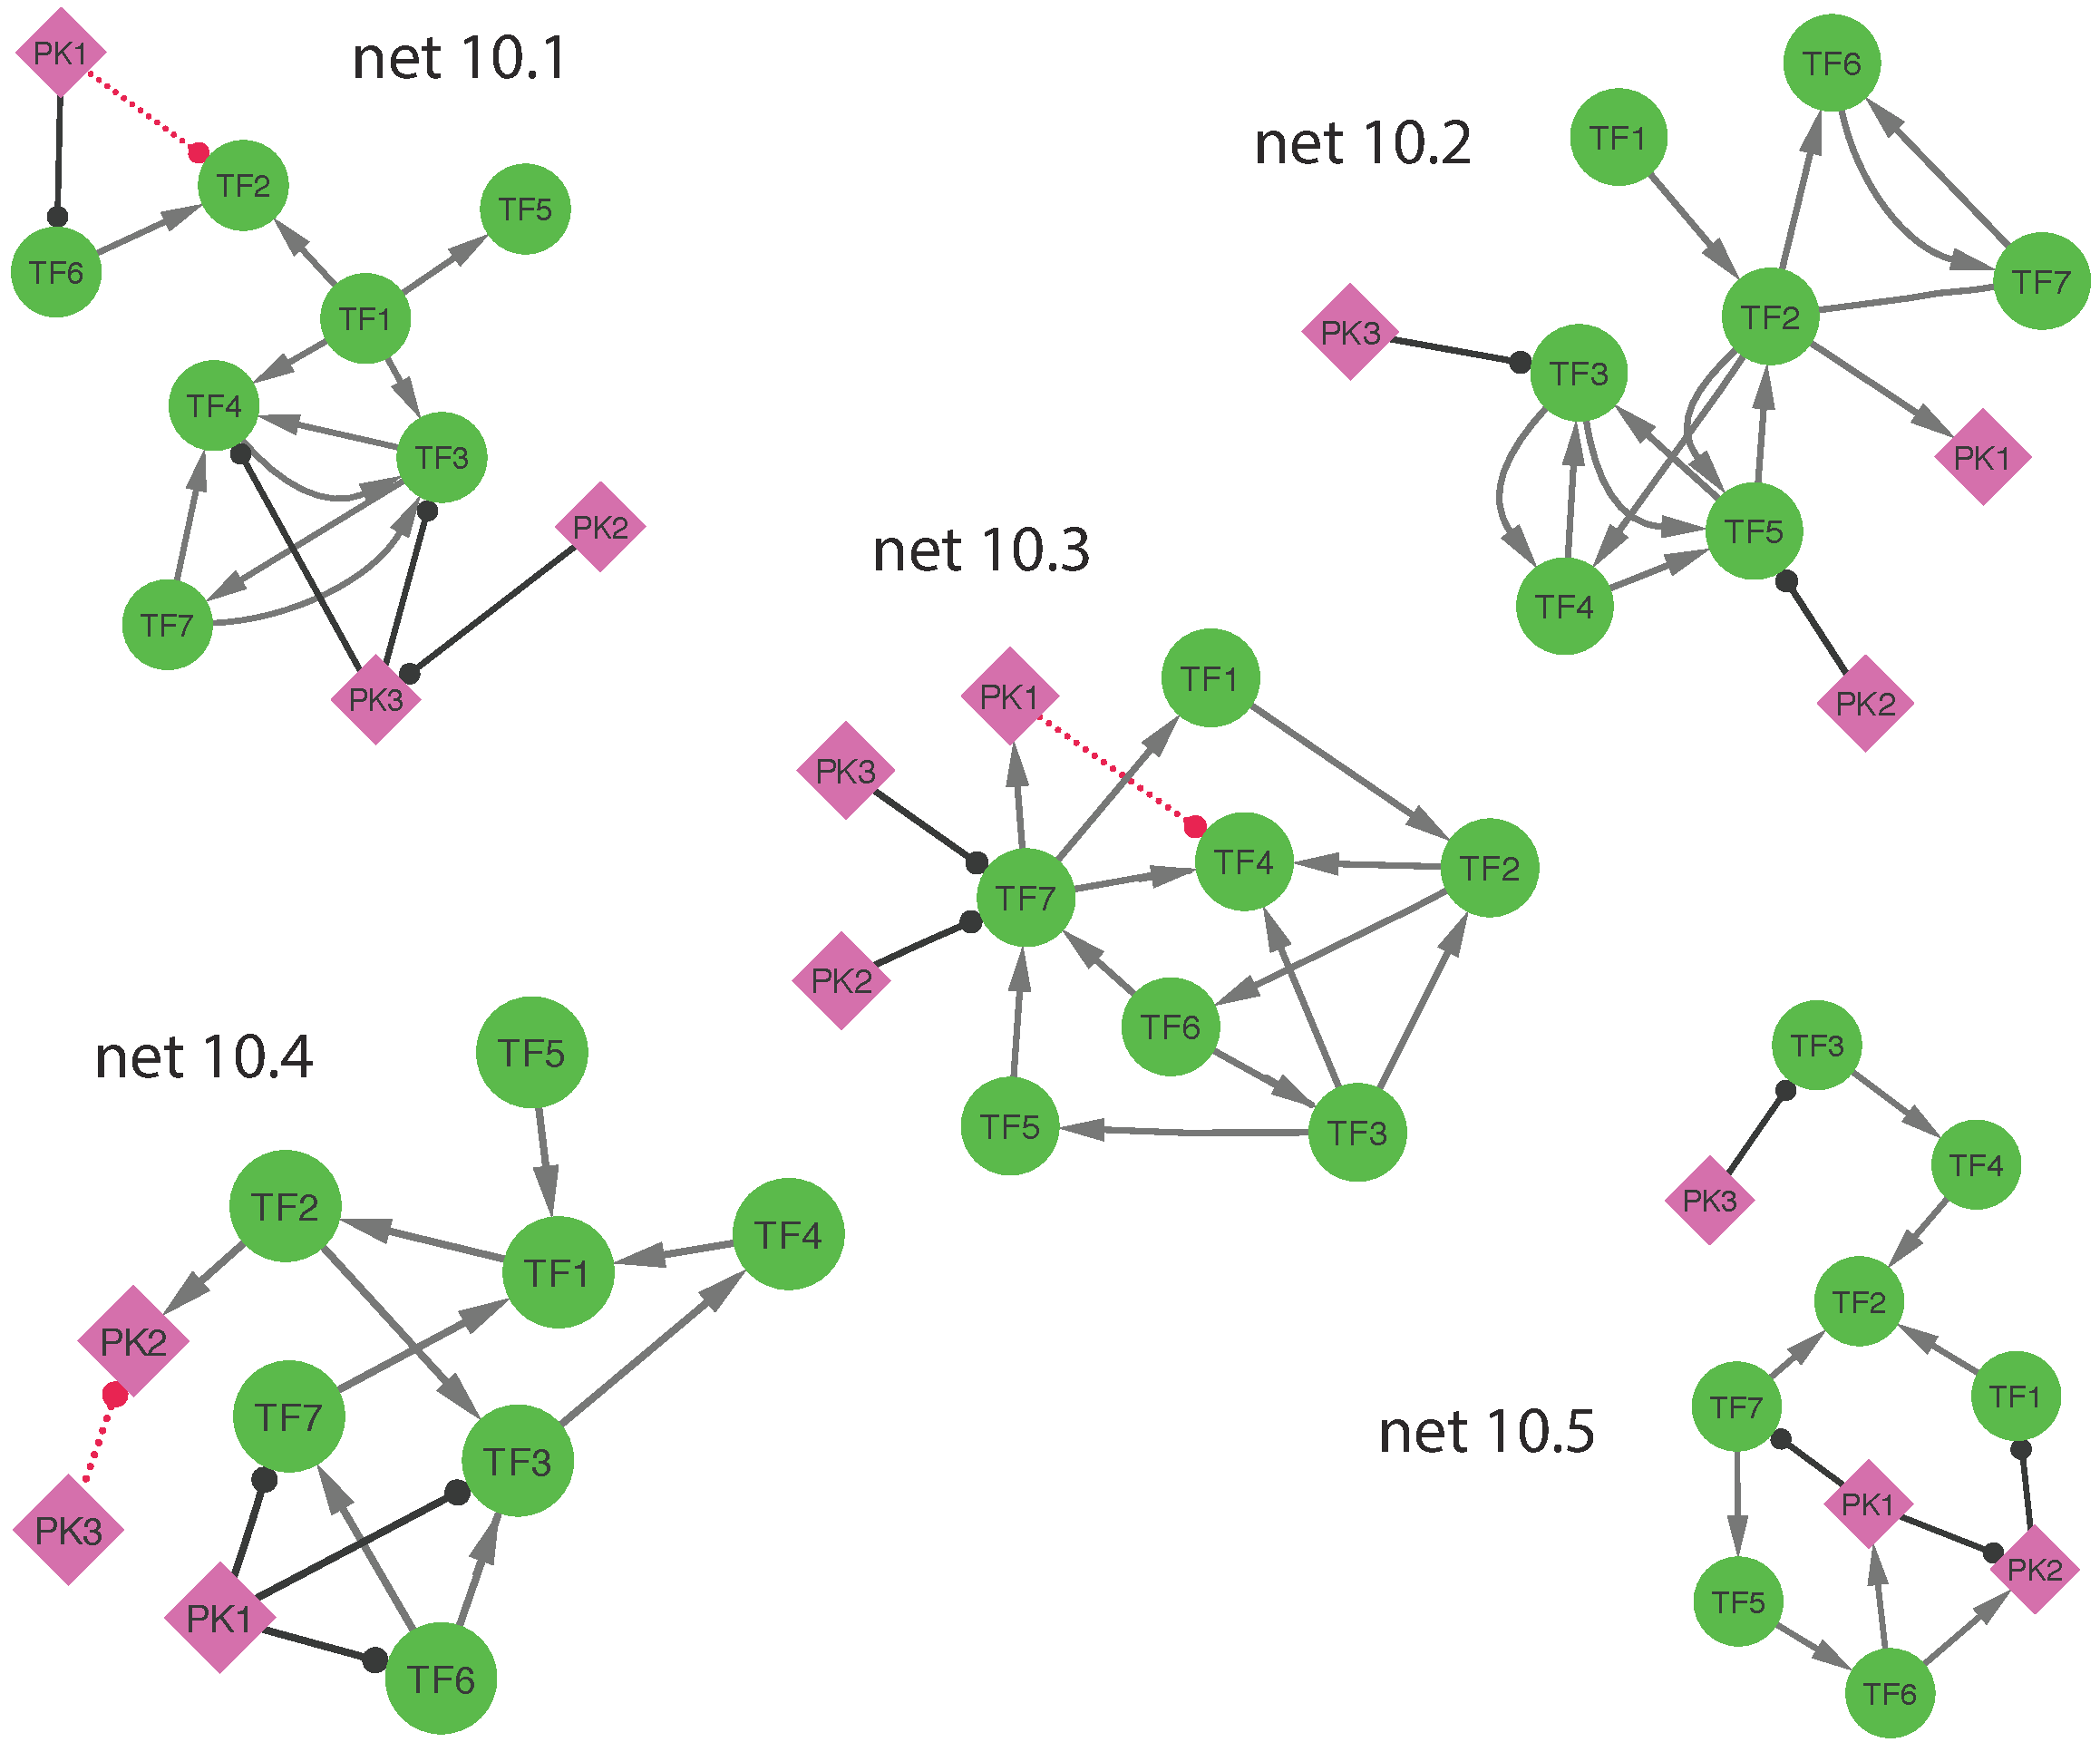
\includegraphics[height=0.85\textheight]{data/fig/nets_10.pdf}
    \caption{\textbf{Networks with 10 nodes.} \textcolor{gray}{Gray} = TF edge, \textcolor{black}{black} = detectable KP edge, \textcolor{red}{red} = silent KP edges. }
    \label{fig:dream4_nets10}
\end{figure}}
{\stepcounter{figure}
\begin{figure}[ht]
    \centering
    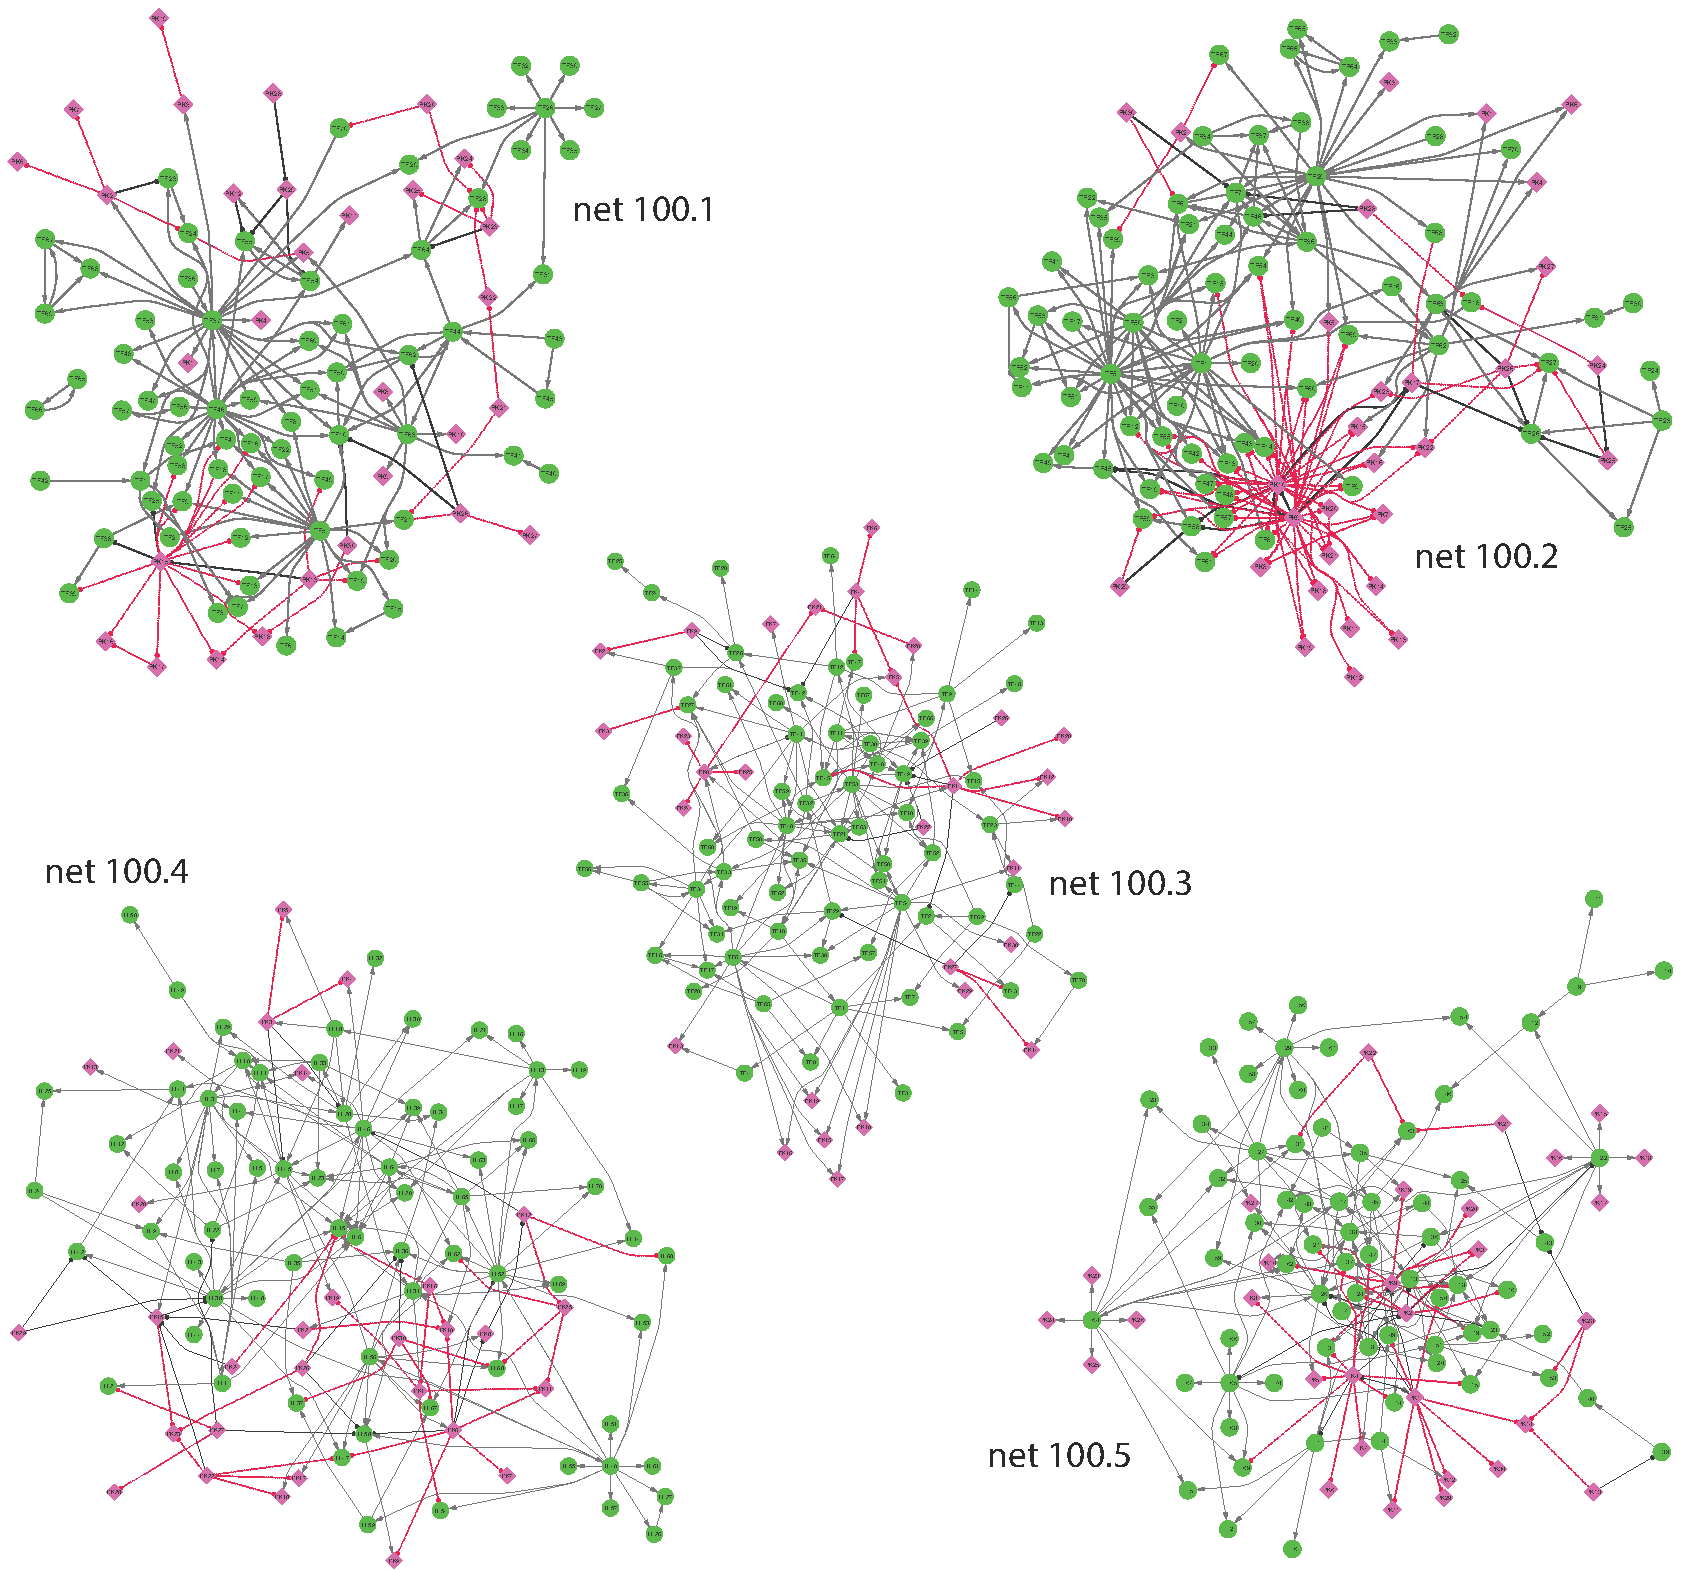
\includegraphics[height=0.85\textheight]{data/fig/nets_100.pdf}
    \caption{\textbf{Networks with 100 nodes.} \textcolor{gray}{Gray} = TF edge, \textcolor{black}{black} = detectable KP edge, \textcolor{red}{red} = silent KP edges. }
    \label{fig:dream4_nets100}
\end{figure}}
% The simulated RNA expression levels are not used since they are simulated using GeneNetWeaver which does not use kinase effects in its gene regulation model. The gold standard true edges are used here. They are given as a list of all pairs of nodes with a 1 or 0 to indicate presence or absence of a directed edge. This was formatted as an adjacency matrix of ones and zeros with edge source nodes as column names and edge target nodes as row names.
% The first~70\% of nodes are used as transcription factors and the remaining~30\% as kinase/phosphatases to roughly match the proportions observed in the yeast data~(\autoref{sec:yeast_data}). So, for 10 node networks there are 7 nodes assigned as TFs and 3 assigned as PKs, for 100 node networks there are 70 assigned as TFs and 30 as PKs.
% The graphs are shown for networks of 10 nodes~(\autoref{fig:dream4_nets10}), for networks of 100 nodes~(\autoref{fig:dream4_nets100}), as well as larger versions of 100 node networks~(\autoref{app:dream_nets}). Each graph are plotted with unsigned edges between TFs and PKs. As discussed in~\autoref{sec:unobservable}, there are certain circumstances where a PK to TF edge will be silent in RNA knockout measurements. These edges are here referred to as undetectable or silent edges.
\end{column}
\end{columns}
\end{frame}

% \begin{frame}{DREAM challenge networks}
% \begin{table}[ht]
% \caption{\textbf{Gold standard networks.} "detectable PK edge" = has effect on gene expression. "detectable PK nodes" = $\ge1$ detectable in- or outgoing edge. "nonsilent PK nodes" = $\ge1$ detectable outgoing edge. }
% \begin{tabularx}{\textwidth}{@{}XXXXXX@{}}
%     \toprule
%     & TF edges & PK edges & \pbox[t]{4cm}{detectable \\ PK edges} & \pbox[t]{4cm}{detectable \\ PK nodes} & \pbox[t]{4cm}{nonsilent \\ PK nodes} \\
%     \midrule
%     net 10.1 & 10 & 5 & 4 & 3 & 3 \\
%     net 10.2 & 14 & 2 & 2 & 3 & 2 \\
%     net 10.3 & 12 & 3 & 3 & 3 & 2 \\
%     net 10.4 & 9 & 4 & 3 & 2 & 1 \\
%     net 10.5 & 8 & 4 & 4 & 3 & 3 \\
%     net 100.1 & 176 & 48 & 13 & 19 & 9 \\
%     net 100.2 & 249 & 101 & 17 & 20 & 9 \\
%     net 100.3 & 195 & 28 & 11 & 23 & 7 \\
%     net 100.4 & 211 & 51 & 19 & 24 & 12 \\
%     net 100.5 & 193 & 52 & 15 & 23 & 7 \\
%     \bottomrule
% \end{tabularx}
% \label{tab:dream_data}
% \end{table}
% % Counts of nodes and edges are summarized in~\autoref{tab:dream_data}. Undetectable edges will not be considered for performance since they will not be detected regardless of inference method. This reduces the effective sizes of the graphs to having the number of PKs listed in column "detectable PK nodes" and to have the PK edges listed in "detectable PK edges".
% % To simulate node values, the gold standard edges are randomly signed and given a random strength. This is generally done by providing a random uniform number in range $[-1,1]$ for each nonzero entry in the gold standard adjacency matrix. It was also tested with standard Gaussian random values.
% % Gene expression levels as log fold-change RNA values are simulated using each of these networks for performance testing of edge inference. Simulation is performed using simple iteration discussed in~\autoref{sec:prim}, or using the GeneNetWeaver extension discussed in~\autoref{sec:gnw_extension}.
% \end{frame}
